\documentclass[12pt]{report}

%Packages-------------------------------------
\usepackage{amsmath}
\usepackage{amsfonts}
\usepackage{amssymb}
\usepackage{amsthm}
\usepackage{graphics}
\usepackage{graphicx}
\usepackage{hyperref}

%\usepackage{xtocnic}

\usepackage{xepersian}

\settextfont{XB Zar}

%Layout---------------------------------------

%\usepackage[top=2cm, bottom=2cm, left=2cm, right=2cm]{geometry}

%Commands-------------------------------------


%Theorems-------------------------------------
\newtheorem{thm}{قضیه}[chapter]
\newtheorem{cor}[thm]{نتیجه}
\newtheorem{defn}[thm]{تعریف}
\newtheorem{prop}[thm]{گزاره}
\newtheorem{lmm}[thm]{لم}
\newtheorem{conj}[thm]{حدس}
\newtheorem{exm}[thm]{مثال}
\newtheorem{rem}[thm]{تذکر}
\newtheorem{note}[thm]{یادداشت}
\newtheorem{alg}[thm]{الگوریتم}


\begin{document}

%Title page ---------------------------------------------

\begin{figure}
\centering

\includegraphics[height=2.5cm]{UT-Logo.pdf}
\end{figure}

\begin{center}
پردیس علوم
\\
دانشکده ریاضی، آمار و علوم کامپیوتر
\end{center}

\begin{center}
%%%%%%%%%%%%%
\end{center}

\begin{center}
\huge{بررسی الگوریتم‌های تکرار بافاصله در یادگیری با فلش‌کارت}
\end{center}

\begin{center}
%%%
\end{center}

\begin{center}
نگارنده
\end{center}
\begin{center}
\textbf{
محمد ترابی}
\end{center}

\begin{center}
\begin{tabular}{rr}
استاد راهنما: دکتر هدیه ساجدی

\end{tabular}
\end{center}

\vspace{3cm}
\begin{center}
پایان‌نامه برای دریافت درجه کارشناسی
\\
در رشته علوم کامپیوتر
\end{center}

\begin{center}
تاریخ: شهریور ۱۴۰۴
\end{center}

\pagestyle{empty}
\pagenumbering{}

\newpage
%\pagestyle{headings}
%\setcounter{page}{1}
%\pagenumbering{roman}
\pagestyle{plain}
\setcounter{page}{1}
\pagenumbering{harfi}
%Abstract page-------------------------------
\chapter*{}
\section*{چکیده}
چکیده پایان‌نامه باید شامل نتایج اصلی مورد مطالعه باشد. توجه نمایید که چکیده با پیشگفتار تفاوت دارد و جای طرح مبانی یا مفاهیم مقدماتی نیست. چکیده تنها باید شامل نتایج و کار اصلی انجام شده در پایان‌نامه باشد. طول چکیده معمولا بیشتر از یک یا دو پاراگراف نیست.

%Dedication page-----------------------------
%\chapter*{تقدیم به}
%\section*{تقدیم به}

%Acknowledgement page------------------------
\chapter*{سپاسگزاری}
صمیمانه از استاد راهنمای گرانقدرم، سرکار خانم دکتر ساجدی، برای راهنمایی‌های ارزشمندشان سپاسگزارم و از جناب آقای دکتر باباعلی، مدیر محترم گروه علوم کامپیوتر، کمال تشکر را دارم. یاد و خاطره استاد ارجمند، مرحوم دکتر نوذری، که دانش و بینش ایشان همواره الهام‌بخش بود، گرامی باد.
%copyright + declaration page
%\chapter*{اصالت اثر}
%\section*{اصالت اثر}
% هیچ قسمت از این پایان‌نامه، پیش از این در هیج موسسه تحصیلات عالی برای دریافت درجه تحصیلی استفاده نشده است. همچنین، هیچ قسمت از این پایان‌نامه برگردان فارسی تمامی یا قسمتی از یک اثر دیگر علمی (مانند مقاله، پایان‌نامه، و غیره) به زبانی دیگر نمی‌باشد. ارائه این پایان‌نامه توسط نگارنده به معاونت آموزشی (معاونت پژوهشی و تحصیلات تکمیلی برای ارشد و دکتری) به منزله تعهد نگارنده به اصالت متن و محتوای ارائه شده بر اساس یک کار پژوهشی در مدت تحصیل در دانشگاه تهران می باشد. در صورت اثبات خلاف این امر، مدرک تحصیلی اخذ شده توسط این پایان‌نامه از دانشگاه تهران، معتبر نمی باشد. 
%
%\chapter*{حق مالکیت معنوی}
%\section*{حق مالکیت معنوی}
%حق مالکیت معنوی این اثر متعلق به دانشگاه تهران می باشد. استفاده از مطالب این پایان‌نامه در فعالیت های تحقیقاتی با ذکر منبع بلامانع می‌باشد. در صورت استفاده تجاری، مانند چاپ این پایان‌نامه، هماهنگی لازم و اجازه کتبی از دانشگاه و نگارنده پایان‌نامه الزامی می‌باشد.

%\listoffigures

%-------------------------
%\pagestyle{plain}
%\setcounter{page}{1}
%\pagenumbering{harfi}
%-------------------------


\chapter*{پیشگفتار }

پیشگفتار، فصلی از پایان‌نامه است که معمولاً شامل بخش یا زیربخش نیست. در این بخش، مقدمه‌ای به زبان ساده و عاری از فرمول‌بندی ریاضی، از مساله مورد مطالعه در پایان‌نامه ارائه می‌شود. نیز در پیشگفتار است که می‌توان خواننده را با تاریخچه‌ای مختصر از تلاش‌هایی که برای حل مساله مورد مطالعه در پایان‌نامه شده است آشنا نمود و نیز تلاش نمود تا خواننده اهمیت کار انجام شده در پایان‌نامه را دریابد. این قسمت، گرچه در نگاه نخست به ظاهر بسیار ساده می‌نماید، اما در حقیقت یکی از  مهمترین قسمت‌های پایان‌نامه است، زیر بازتاب دهنده دانسته‌ها و فهم دانشجو از کلیت مساله است. توصیه می‌کنیم که نوشتن این قسمت را به آخر موکول نمایید!
\\
یک نکته مهم: اگر پایان‌نامه یک پایان‌نامه کارشناسی یا کارشناسی‌ارشد باشد، که معمولاً بر اساس یک یا چند مقاله نوشته می‌شوند، آنگاه از دانشجو انتظار می‌رود که مراجع اصلی خود را در پیشگفتار معرفی نماید.
\\
معمولاً بخش آخر پیشگفتار به ارائه یک نمایه کلی از پایان‌نامه اختصاص می‌یابد و نگارنده به معرفی کوتاهی از فصل‌بندی و کار انجام شده در پایان‌نامه می‌پردازد.

\tableofcontents

\chapter{مفاهیم مقدماتی}

%---------------------
\pagestyle{plain}
\setcounter{page}{1}
\pagenumbering{arabic}
%---------------------


% یک پایان‌نامه ریاضی، معمولاً شامل تعاریف و مفاهیم تخصصی می‌باشد. توصیه می‌شود که فصلی از پایان‌نامه به معرفی مفاهیم مقدماتی که در پایان‌نامه به کار رفته‌اند اختصاص یابند. معمولاً نمادگذاری و معرفی کلیدواژه‌های به کار رفته در پایان‌نامه در این فصل انجام می‌پذیرد و یک خواننده عادی، داور پایان‌نامه، یا هر شخص دیگری در صورت عدم آشنایی با مفهومی می‌تواند به این فصل مراجعه نماید. توصیه می‌کنیم که این معرفی و نمادگذاری به زبانی روان و گویا انجام پذیرد و نیز با توجه به تفیکیک موصوعات و ارتباط منطقی بین آنها انجام پذیرد. معمولاً هر فصل، به غیر از پیشگفتار، شامل بخش‌ها و زیر بخش‌هایی می‌باشد که می‌توانند بر اساس تقسیم‌بندی موضوعی صورت پذیرند. برای نمونه برای مطالعه یک مطلب درباره سیستم‌های دینامیکی ناخودگرد، وجود یک بخش درباره سیستم‌های دینامیکی در حالت کلی و نیز بخش یا زیربخشی درباره حالت ناخودگردی یک تقسیم‌بندی مناسب به نظر می‌آید.

% توجه کنید که لزومی به اثبات همه مطالب و قضیه‌های مقدماتی، در این فصل، نیست و اصولاً چنین کاری شیوه مرسوم نیست. معمولاً انتخاب و ارجاع خواننده به یک کتاب معتبر یا هر مرجع معتبر دیگری بسیار مناسب‌تر است. چنین فصلی، جایی مناسب برای قضیه‌های "کلاسیک" درباره مساله مورد مطالعه می‌باشد. توجه کنید که یک قضیه می‌تواند صورت‌های مختلفی داشته باشد و بهتر است از آن صورت مورد استفاده خود در این قسمت استفاده نمایید!

\section{فلش‌کارت چیست؟}
فلش‌کارت‌ها ابزاری ساده اما بسیار 
\textbf{کارآمد}
برای یادگیری و به‌خاطرسپاری اطلاعات هستند. این ابزارها، که می‌توانند به شکل 
کاغذی یا الکترونیکی باشند، شامل مجموعه‌ای از کارت‌ها هستند
 که روی یک یا هر دو طرف آن‌ها اطلاعاتی نوشته شده است. از فلش‌کارت‌ها 
می‌توان برای یادگیری طیف گسترده‌ای از موضوعات استفاده کرد، از جمله:

\begin{itemize}
  \item \textbf{زبان‌های خارجی}: یادگیری واژگان جدید
  \item \textbf{علوم پایه}: به‌خاطر سپردن مطالب در دروس پزشکی، حقوق، تاریخ و جغرافیا
  \item \textbf{مهارت‌های تخصصی}: حفظ نت‌های گیتار، اصطلاحات علوم کامپیوتر\\ یا مرور یادداشت‌های مهم
  \item \textbf{موارد روزمره}: به‌خاطر سپردن نام افراد از روی تصویرشان
\end{itemize}

\section{تکرار بافاصله
\protect\footnote{\lr{Spaced Repetition}}
}

برای ماندگاری بیشتر اطلاعات در حافظه، مرور مطالب ضروری است.
\textbf{تکرار بافاصله}
 روشی است که در آن مرور مطالب در فواصل زمانی مشخص و بهینه انجام می‌شود.
  این فواصل با گذشت زمان،
  به‌تدریج طولانی‌تر می‌شوند. 
 این شیوه بر اساس الگوریتم‌هایی 
 طراحی شده است که بهترین زمان را
  برای تکرار هر مطلب محاسبه می‌کنند. 
 با استفاده از این روش، اثربخشی
  یادگیری به‌طور چشمگیری افزایش می‌یابد. 
 در این مقاله چند الگوریتم مرتبط
  با تکرار بافاصله را 
 بررسی خواهیم کرد.

% در یک پایان‌نامه ریاضی، انواع گزاره‌ها برای بیان مطالب و مفاهیم به کار می‌رود. عناوینی مانند، قضیه، گزاره، لم، حکم، الگوریتم، اثبات، مثال، تذکر، یادآوری، یادداشت، حدس و غیره. توصیه اکید می‌کنیم که از صورت کلی زیر برای ایجاد محیط مناسب استفاده نمایید
% \begin{latin}
% \[
% \begin{array}{l}
% \backslash\textrm{begin\{env. name\}}\\
% \\
% \backslash\textrm{end\{env. name\}}
% \end{array}
% \]
% \end{latin}
% در زیر جدولی از محیط های تعریف شده آمده است

% \begin{center}
% \begin{tabular}{c|c}
% محیط تعریف شده & env. name
% \\

% \hline

% \\
% قضیه& thm
% \\
% گزاره یا حکم & prop
% \\
% لم & lmm
% \\
% تعریف & defn
% \\
% مثال & exm
% \\ 
% تذکر & rem
% \\ 
% یادداشت & note
% \\
% الگوریتم & alg
% \\
% اثبات & proof
% \end{tabular}
% \end{center}

% برای نمونه تعریف زیر با استفاده از محیط 
% $$\begin{array}{l}
% \backslash\textrm{begin\{defn\}} \\ \\
% \backslash\textrm{end\{defn\}}
% \end{array}$$
% ایجاد شده است.
% \begin{defn}
% عدد طبیعی 
% $p$، 
% $p\neq 1$، 
% را اول گوییم، هرگاه به غیر از خودش و یک مقسوم علیه دیگری نداشته باشد.
% \end{defn}

\section{منحنی فراموشی \protect\footnote{\lr{Forgetting Curve}}}
\textbf{منحنی فراموشی}
نموداری است که نشان می‌دهد چگونه میزان به‌خاطرآوردن 
مطالب در طول زمان کاهش می‌یابد.
 این نمودار توسط روانشناس آلمانی،
 هرمان ابینگهاوس
\footnote{\lr{Hermann Ebbinghaus (1850–1909)}}
 ، معرفی شد. محور 
افقی این نمودار نشان‌دهنده زمان و
 محور عمودی آن،
\textbf{میزان یادآوری}
\footnote{Retention} یا احتمال به‌خاطرآوردن مطلب است.

همانطور که در
شکل~\ref{fig:forgetting-curve}
مشخص است، اگر مطالب مرور نشوند،
 میزان یادآوری به‌سرعت کاهش می‌یابد.
 اما با استفاده از تکرار بافاصله،
 همانطور که در
شکل~\ref{fig:forgetting-curve-with-repetition}
 دیده می‌شود،
 شیب منحنی پس از هر بار مرور کمتر می‌شود.
 این بدان معناست که با هر بار تکرار،
 مدت‌زمان بیشتری طول می‌کشد تا مطلب فراموش شود
 و نیاز به مرور کمتری پیدا می‌کند.
 
\begin{figure}[h!]
  \centering
  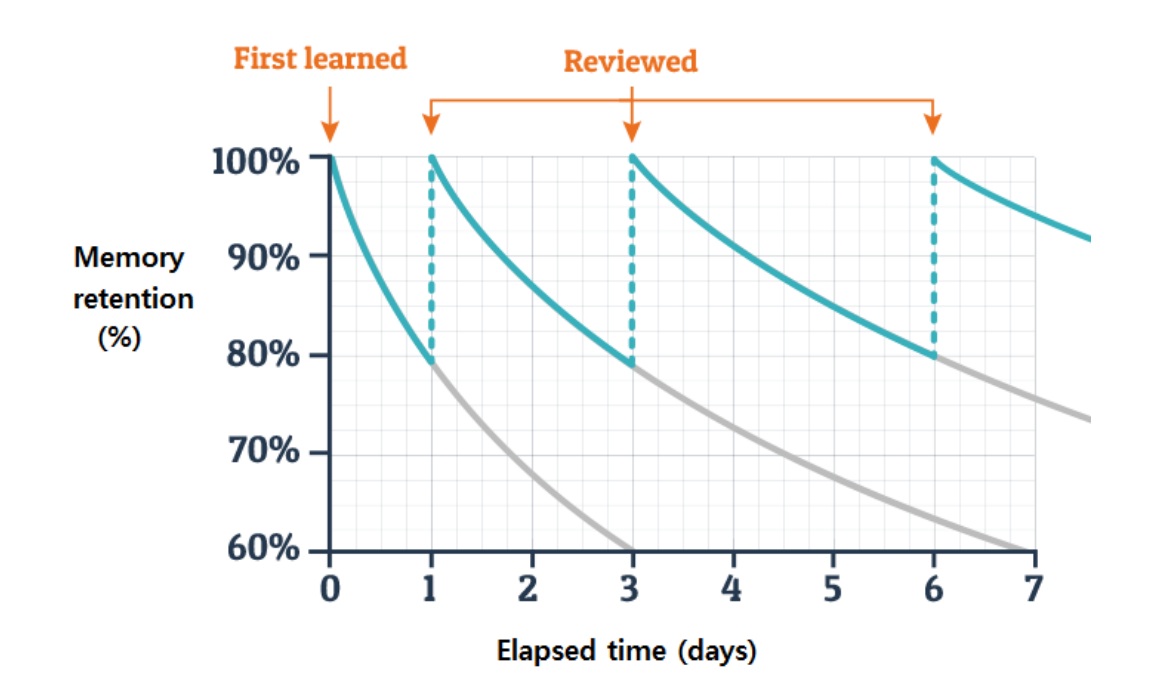
\includegraphics[width=0.8\textwidth]{images/forgetting-curve.png}
  \caption{منحنی فراموشی بدون مرور مطالب}
  \label{fig:forgetting-curve}
\end{figure}

\begin{figure}[h!]
  \centering
  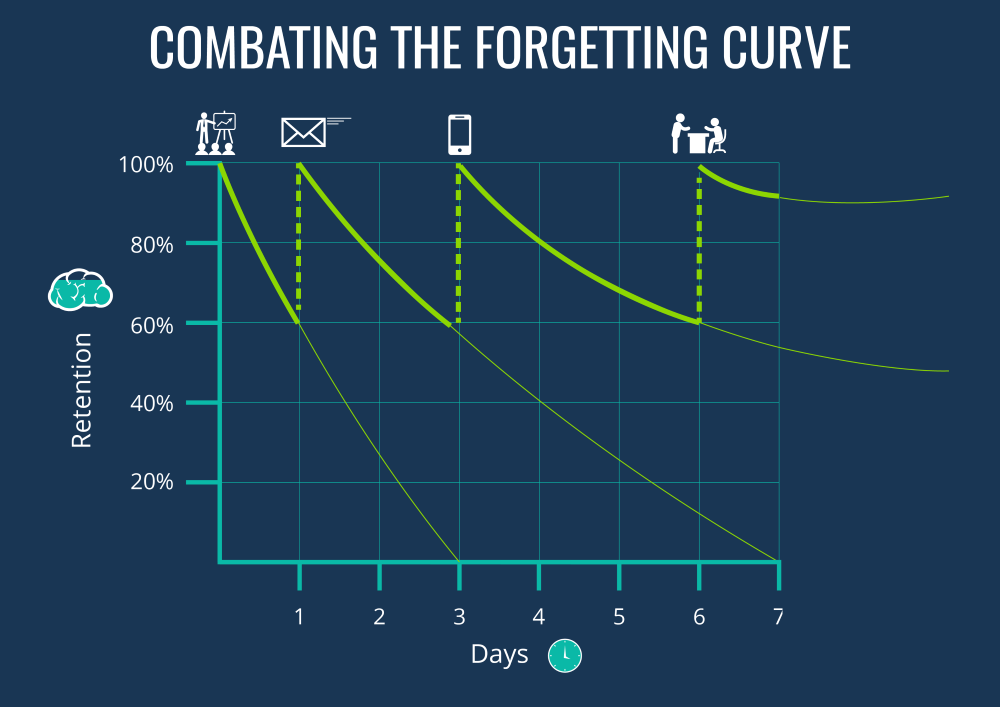
\includegraphics[width=0.8\textwidth]{images/forgetting-curve-with-repetition.png}
  \caption{منحنی فراموشی با مرور مطالب}
  \label{fig:forgetting-curve-with-repetition}
\end{figure}

\chapter{اصول طراحی فلش‌کارت‌های کارآمد}


\section{ویژگی‌های یک فلش‌کارت خوب}

% ایجاد لیست شماره‌دار با استفاده از محیط enumerate
\begin{enumerate}
    \item \textbf{طراحی به شکل پرسش و پاسخ:} بهترین فلش‌کارت‌ها از شما می‌خواهند به جای مرور صرف، به یک سوال پاسخ دهید. تحقیقات نشان داده‌اند که \textbf{یادآوری فعال}\footnote{\lr{Active Recall}}، یعنی تلاش برای بازیابی اطلاعات، به یادگیری عمیق‌تر و ماندگارتر منجر می‌شود. این پدیده به «\textbf{اثر آزمون}»\footnote{\lr{Testing Effect}} نیز معروف است.

    \item \textbf{کوتاه و مختصر:} یک فلش‌کارت باید شامل یک مفهوم یا واقعیت واحد باشد. مطالب کوتاه‌تر، یادگیری را ساده‌تر کرده و امکان مرور متناسب با میزان سختی هر بخش را فراهم می‌کنند. در مقابل، کارت‌های شلوغ مجبورمان می‌کنند کل محتوا را تکرار کنیم، حتی اگر بخشی از آن را بلد باشیم.

    \item \textbf{اجتناب از فهرست‌ها:} به جای پرسیدن "کشورهای خاورمیانه را نام ببرید؟"، بهتر است هر کشور را در یک کارت جداگانه با سوالات خاصی مانند "بزرگ‌ترین کشور خاورمیانه کدام است؟" یا "ثروتمندترین کشور آن کدام است؟" یاد بگیرید. این کار از ناکارآمدی حفظ فهرست‌های بلند جلوگیری می‌کند. سپس می‌توانید با پیوند دادن این اطلاعات، به سوال اصلی پاسخ دهید.
    
    \item \textbf{منابع بیشتر:} برای آشنایی با ویژگی‌های دقیق‌تر و قوانین بهینه‌سازی فلش‌کارت‌ها، می‌توانید به مقالهٔ 
    «\href{https://super-memory.com/articles/20rules.htm}{بیست قانون برای فرمول‌بندی دانش}»
\footnote{\lr{Twenty Rules of Formulating Knowledge}}
    مراجعه کنید. این مقاله توسط پاوو اولکوفسکی، بنیان‌گذار الگوریتم \lr{SuperMemo}، نوشته شده است.
\end{enumerate}

\section{مزایا و معایب مطالعه با فلش‌کارت‌ها}


\subsection{مزایا}
\begin{itemize}
    \item \textbf{افزایش ماندگاری:} با استفاده از تکرار بافاصله، مطالب برای مدت‌زمان طولانی‌تری در حافظه می‌مانند.
    \item \textbf{یادگیری فعال:} فلش‌کارت‌ها به دلیل ماهیت پرسش و پاسخ خود، یادگیری را فعال کرده و به جای مرور صرف، به یادآوری و بازیابی اطلاعات کمک می‌کنند.
    \item \textbf{تمرکز بر نقاط ضعف:} با طبقه‌بندی کارت‌ها بر اساس میزان سختی، می‌توان روی مطالبی که تسلط کمتری بر آن‌ها دارید، بیشتر تمرکز کرد.
    \item افزایش انگیزه یادگیری به دلیل ساده و بازی‌گونه بودن و امارها و اینکه می‌بینیم چقدر پیشرفت کردیم.
\end{itemize}

\subsection{معایب}
\begin{itemize}
    \item \textbf{زمان‌بر بودن:} تهیه فلش‌کارت‌ها ممکن است زمان‌بر باشد، هرچند ابزارهای الکترونیکی این فرایند را ساده‌تر کرده‌اند.
    \item \textbf{نیاز به نظم و انضباط:} اثربخشی این روش به مرور منظم و مداوم وابسته است.
\end{itemize}

\chapter{اصول طراحی الگوریتم‌های تکرار بافاصله}

\section{ویژگی‌های کلیدی یک الگوریتم تکرار خوب}
یک الگوریتم تکرار خوب، برای بهینه‌سازی فرآیند یادگیری، باید ویژگی‌های زیر را داشته باشد. که البته داشتن همه این موارد کار سختی است.

\begin{enumerate}
    \item \textbf{محاسبه بهینه فواصل تکرار:} هدف اصلی الگوریتم، یافتن \textbf{بهترین زمان تکرار} برای هر کارت است. این زمان باید طوری باشد که کارت درست قبل از اینکه فراموش شود، دوباره نمایش داده شود. این کار باعث می‌شود با \textbf{کمترین تعداد مرور}، اطلاعات برای \textbf{بیشترین زمان ممکن} در حافظه باقی بماند.

    \item \textbf{توزیع بار مرور:} یک الگوریتم هوشمند باید از \textbf{انباشته شدن فلش‌کارت‌ها} در یک روز خاص جلوگیری کند. به عبارت دیگر، وظیفه آن \textbf{توزیع بهینه} کارت‌ها در طول زمان است تا کاربر هر روز حجم معقول و مدیریت‌پذیری از کارت‌ها را برای مرور داشته باشد و از احساس خستگی یا عقب‌افتادگی جلوگیری شود. یعنی حجم فلش‌کارت‌ها در یک روز نباید خیلی کم و یا خیلی زیاد باشد.

    \item \textbf{تطبیق با سختی مطالب:} الگوریتم باید بر اساس عملکرد کاربر و \textbf{سختی و آسانی} هر کارت، فواصل تکرار را تنظیم کند. برای کارت‌های آسان‌تر، فاصله زمانی بیشتر می‌شود و برای کارت‌های دشوار، مرور در فواصل کوتاه‌تری انجام می‌گیرد. این ویژگی، فرآیند یادگیری را شخصی‌سازی کرده و کارآمدتر می‌کند.

    \item \textbf{سازگاری با مطالعه نامنظم:} یک الگوریتم قوی باید با \textbf{مطالعه نامنظم} سازگار باشد و در صورت وقفه طولانی، دچار اختلال نشود. اگر کاربری برای چند روز یا هفته مطالعه نکند و سپس مرور را از سر بگیرد، الگوریتم باید این وقفه را درک کرده و فواصل زمانی را به‌درستی تنظیم کند. برای مثال، اگر قرار بود کارتی امروز مرور شود و سپس یک هفته بعد نمایش داده شود اما کاربر به جای امروز پس از یک ماه آن را مرور می‌کند، الگوریتم باید این فاصله زمانی طولانی را به عنوان یک "یادآوری موفق" ثبت کند و فاصله بعدی را بر اساس این واقعیت جدید، به جای یک هفته، به مراتب طولانی‌تر تعیین نماید.
\end{enumerate}

\section{بازه‌های زمانی بهینه}

ممکن است تصور کنیم هر نوع بازه‌ی زمانیِ افزایشی برای مرور مناسب است. 
«وزنیاک» برای بررسی همین موضوع آزمایشی طراحی کرد، اما برخلاف انتظارش نتیجه چیز دیگری شد.
او تعدادی فعل بی‌قاعده‌ی انگلیسی را به سه گروه تقسیم کرد و هر گروه را با فواصل زمانی متفاوت مرور کرد.
 در هر کارت، فعل روی کارت نوشته شده بود و سه شکل صرف آن پشت کارت قرار داشت.
هر گروه شش بار مرور شد.
برنامه زمانی مرور هر گروه در جدول~\ref{tbl:repetition_schedule} آمده است.


\begin{table}[h!]
    \centering
    \caption{برنامه زمانی مرور گروه‌های آزمایشی}
    \label{tbl:repetition_schedule}
    \begin{tabular}{|c|c|c|c|}
        \hline
        نوبت مرور & گروه A & گروه B & گروه C \\
        \hline
        ۱ & ۱۸ روز & ۱ روز & ۵ روز \\
        \hline
        ۲ & ۱۸ روز & ۵ روز & ۵ روز \\
        \hline
        ۳ & ۱۸ روز & ۹ روز & ۵ روز \\
        \hline
        ۴ & ۱۸ روز & ۲۴ روز & ۵ روز \\
        \hline
        ۵ & ۱۸ روز & ۴۴ روز & ۵ روز \\
        \hline
        ۶ & ۱۸ روز & ۷۰ روز & ۵ روز \\
        \hline
        مجموع & ۱۰۸ روز & ۱۵۳ روز & ۳۰ روز \\
        \hline
    \end{tabular}
\end{table}

\chapter{الگوریتم لایتنر}

\chapter{الگوریتم \lr{SuperMemo}}

\chapter{عنوان فصل}

\chapter{نتیجه گیری}

\chapter*{واژه‌نامه فارسی به انگلیسی}

\chapter*{ واژه‌نامه انگلیسی به فارسی}

\begin{thebibliography}{MM}
\bibitem{one}
\end{thebibliography}

\begin{latin}
\begin{abstract}
Abstract goes here...
\end{abstract}
\newpage
\thispagestyle{empty}
%Title page ---------------------------------------------
\begin{figure}
\centering

\includegraphics[height=2.5cm]{UT-Logo.pdf}
\end{figure}
\begin{center}

College of Science\\
School of Mathematics, Statistics, and Computer Science
\end{center}

\begin{center}
%%%%%%%%%%%%%
\end{center}

\begin{center}
\huge{Title of the Project}
\end{center}

\begin{center}
%%%
\end{center}

\begin{center}
\textbf{
Mohamamd Torabi
}
\end{center}

\begin{center}
Supervisor: Dr.\ Hedieh Sajedi
\end{center}

\vspace{3cm}
\begin{center}
A thesis submitted in partial fulfillment of the requirements for\\
the degree of B.Sc.\ in Computer Science
\end{center}

\begin{center}
2025
\end{center}

%\pagestyle{empty}
%\pagenumbering{}

\end{latin}

\end{document}
